\documentclass[12pt]{article}
\usepackage[brazil]{babel}
\usepackage{graphicx}
\usepackage{mathtools}
\usepackage{float} 
\usepackage{xcolor}
\usepackage{amsmath, amssymb, bm}


\usepackage{array}
\usepackage{booktabs}



% margenes
\usepackage[a4paper,left=3cm,right=3cm,top=3cm]{geometry}

%opening
\title{}
\author{}

\begin{document}

\begin{center}
	{\tiny {\normalsize {\large \textbf{Convecção}\\ Lista de exercicios 4\\
	
	\textbf{Cristian Herledy Lopez Lara}}}}
\end{center}

\subsection*{Exercício 1}


\textbf{Determine o número de Nusselt para uma esfera isotérmica $(Ts)$ de diâmetro $D$ envolta por um fluido quiescente mantido a $Tf (Ts < Tf)$ no limite onde o número de Rayleigh baseado em $D$ tende a zero.}\\

\begin{figure}[H]
	\centering
	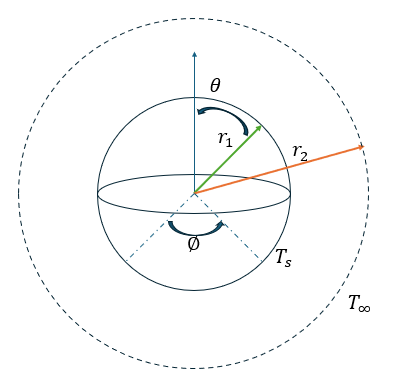
\includegraphics[width=.65\textwidth]{Figures/1_1}
	\caption{Diagrama esfera envolta por fluido quiecente com coordenadas esfericas}
\end{figure}

\textbf{Desenvolvimento} 


Partindo da análise do problema com a equação de conservação de energia


\begin{equation}
	\begin{aligned}
		\rho c_P \left( \frac{\partial T}{\partial t} + v_r \frac{\partial T}{\partial r} + \frac{v_\phi}{r} \frac{\partial T}{\partial \phi} + \frac{v_\theta}{r \sin \phi} \frac{\partial T}{\partial \theta} \right) \\
		= k \left[ \frac{1}{r^2} \frac{\partial}{\partial r} \left( r^2 \frac{\partial T}{\partial r} \right) + \frac{1}{r^2 \sin \phi} \frac{\partial}{\partial \phi} \left( \sin \phi \frac{\partial T}{\partial \phi} \right) + \frac{1}{r^2 \sin^2 \phi} \frac{\partial^2 T}{\partial \theta^2} \right]
	\end{aligned}
\end{equation} \\



Considerando que há simetria da esfera nas direções $\phi , \theta$ e como o fluido está quiescente

\begin{equation}
	\begin{aligned}
		 \frac{1}{r^2} \frac{\partial}{\partial r} \left( r^2 \frac{\partial T}{\partial r} \right) = 0 
	\end{aligned}
\end{equation}

Integrando para encontrar T como uma função do r


\begin{equation}
	\begin{aligned}
		\int \frac{1}{r^2} \frac{\partial}{\partial r} \left( r^2 \frac{\partial T}{\partial r} \right)dr = 0 
	\end{aligned}
\end{equation}


\begin{equation}
	\begin{aligned}
		 \left( r^2 \frac{\partial T}{\partial r} \right) + C_{1} = 0
	\end{aligned}
\end{equation}

Integrando novamente

\begin{equation}
	T = -\frac{1}{r}C_{1} + C_{2}
\end{equation}

As condiçoes de contorno são

\begin{equation}
	 @ r = r_{1} , T = Ts \ ; \ @r = r2, T = T_{inf} 
\end{equation}


\begin{equation}
	C_{1} =  (T_{inf}-Ts ) r_{1} \ \therefore \ C_{2} = T_{inf} 
\end{equation}

Usando a lei de Fourier e a equação de transferência de calor por convecção para equilibrar a troca de energia entre a esfera e o fluido

\begin{equation}
	q'' = h\Delta T = -k \frac{dT}{dr}\arrowvert_{r = r1} 
\end{equation}
Calculando a derivada

\begin{equation}
	\frac{dT}{dr}\arrowvert_{r = r1} = (Ts - T_{inf})\frac{r_{1}}{r^{2}}\arrowvert_{r = r2}
\end{equation}
Sustituindo em (8)


\begin{equation}
	h\Delta T = k \frac{(Ts - T_{inf} ) }{r_{1}}
\end{equation}

Da definição para o numero de Nusselt

\begin{equation}
	Nu_{D} = \frac{hD}{k} \ \rightarrow \  h = \frac{Nu_{D}K}{D}
\end{equation}

Em (10) fica então ($D = 2r_{1}$)

\begin{equation}
	\frac{q''D}{\Delta T k} = k \frac{(Ts - T_{inf} ) }{r_{1}}\frac{2r_{1}}{k (Ts - T_{inf} )}
\end{equation}

\begin{equation}
	Nu_{D} = 2
\end{equation}


Observa-se que o número de Nusselt não depende de nenhuma variável do fluxo. Portanto, devido à velocidade zero do fluido, a transferência de calor da esfera para o fluido é um processo dominado pela condução, onde o calor viaja por convecção da superfície da esfera $T_{s}$ até atingir $T_{inf}$.








\subsection*{Exercício 4.17}


\textbf{Cálculo do tempo de resfriamento de uma garrafa em um refrigerador na posição vertical e horizontal por análise de escala}\\

\begin{figure}[H]
	\centering
	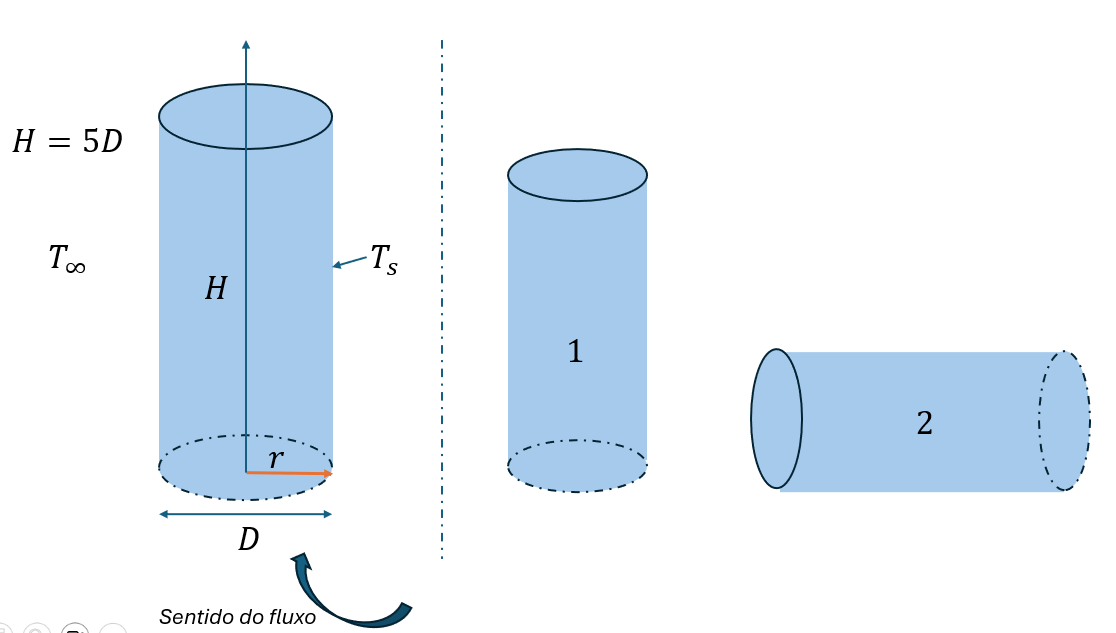
\includegraphics[width=.65\textwidth]{Figures/1_2}
	\caption{Diagrama garrafa em coordenadas cilindricas, e posiçoes vertical e horizontal}
\end{figure}


\textbf{Desenvolvimento} 

Primeiro, as equações constitutivas para o problema são estabelecidas.
Ecuação  de continuidad

\begin{equation}
	\begin{aligned}
		\frac{\partial v_{r}}{\partial r} + \frac{ vr}{ r} + \frac{1 }{ r}\frac{\partial v_{z}}{\partial z} = 0
	\end{aligned}
\end{equation}

Ecuação  de momento em Z

\begin{equation}
	\begin{aligned}
		v_{r}\frac{\partial v_{z}}{\partial r} + v_{z}\frac{\partial v_{z}}{\partial z} = -\frac{1}{\rho} \frac{\partial P}{\partial z} + \nu \left[ \frac{1}{r} \frac{\partial}{\partial r}\left( r\frac{\partial vz}{\partial r}\right) + \frac{\partial^{2}v_{z}}{\partial z} \right] - \rho g 
	\end{aligned}
\end{equation}

Ecuação  de energia

\begin{equation}
	\begin{aligned}
		v_{r}\frac{\partial T}{\partial r} + v_{z}\frac{\partial T}{\partial z} =  \alpha \left[ \frac{1}{r} \frac{\partial}{\partial r}\left( r\frac{\partial vz}{\partial r}\right) + \frac{\partial^{2}T}{\partial z} \right] 
	\end{aligned}
\end{equation}

Como a espessura da camada limite térmica é consideravelmente menor que o comprimento característico do problema $\delta_{t} \ll H$,


\begin{equation}
	\begin{aligned}
		\frac{\partial }{\partial r} \gg \frac{\partial }{\partial z} 
	\end{aligned}
\end{equation}

Considerando que o efeito da pressão é proporcional ao gradiente de pressão hidrostática, que apenas os termos que dependem da direção radial são levados em consideração no operador $\triangledown$ de difusão e que fazendo uso da definição do coeficiente de expansão volumétrica


Ecuação  de momento em Z

\begin{equation}
	\begin{aligned}
		v_{r}\frac{\partial v_{z}}{\partial r} + v_{z}\frac{\partial v_{z}}{\partial z} = + \nu \left[ \frac{1}{r} \frac{\partial}{\partial r}\left( r\frac{\partial vz}{\partial r}\right) \right] + g\beta (T-T_{\infty})
	\end{aligned}
\end{equation}

Ecuação  de energia

\begin{equation}
	\begin{aligned}
		v_{r}\frac{\partial T}{\partial r} + v_{z}\frac{\partial T}{\partial z} =  \alpha \left[ \frac{1}{r} \frac{\partial}{\partial r}\left( r\frac{\partial vz}{\partial r}\right) \right] 
	\end{aligned}
\end{equation}

Com uma análise de escala verifica-se que $( T-T_{\infty} \sim \Delta T)$, $z \sim H$, $r \sim\delta_{T} $, $v_{r}\sim U$

\begin{equation}
	\begin{aligned}
		\frac{g\beta\Delta T \delta_{t}^{2}}{\nu}\sim\frac{H}{\delta_{t}^{2}}
	\end{aligned}
\end{equation}

\begin{equation}
	\begin{aligned}
		 \delta_{t}^{4} \sim \left( \dfrac{\alpha H \nu}{g\beta\Delta T}\right)^{\frac{1}{4}} 
	\end{aligned}
\end{equation}

Como $Nu \sim \frac{H}{\delta_{t}}$

\begin{equation}
	\begin{aligned}
		Nu \sim \left( \dfrac{g\beta \Delta T H^{3} \nu}{\nu \alpha}\right)^{\frac{1}{4}} 
	\end{aligned}
\end{equation}

Onde para fluidos com Prandtl maior que a unidade $Nu \sim Ra^{\frac{1}{4}}$.



Agora, o intercambio do calor entre o ar e a garrafa obedece ao equilíbrio da primeira lei da termodinâmica onde

\begin{equation}
	\begin{aligned}
		\dot{m} C_{p} \frac{dT}{dt} = hA(T_{s}-T_{inf})
	\end{aligned}
\end{equation}

Onde $h$ é o coeficiente de trasnferencia de calor, $A  (A= 2\pi rH + 2\pi r^{2})$ é a área superficial do cilindoO objetivo é encontrar uma relação entre o tempo de resfriamento e a troca de calor convectiva (lado direito da equação) para as posições 1 e 2. Considerando que o calor removido em ambos os arranjos é o mesmo

\begin{equation}
	\begin{aligned}
		Q_{1} = Q_{2}
	\end{aligned}
\end{equation}

\begin{equation}
	\begin{aligned}
		h_{1}A_{1}(T_{s}-T_{inf})t_{1} = h_{2}A_{2}(T_{s}-T_{inf})t_{2}
	\end{aligned}
\end{equation}

\begin{equation}
	\begin{aligned}
		\frac{t_{1} }{t_{2}}= \frac{h_{2}A_{2}}{h_{1}A_{1}}
	\end{aligned}
\end{equation}

Para análise de escala, a área do cilindro na posição vertical e horizontal é proporcional a $H$

\begin{equation}
	\begin{aligned}
		A \sim H \ \ ; \ \ \frac{H_{1}}{H_{2}} = 5
	\end{aligned}
\end{equation}

Pela definição do número de Nusselt

\begin{equation}
	\begin{aligned}
		Nu_{H} = \left( \frac{hH}{k}\right) \sim Ra^{\frac{1}{4}}
	\end{aligned}
\end{equation}
\begin{equation}
	\begin{aligned}
		 h \sim \frac{Ra^{\frac{1}{4}}k}{H}
	\end{aligned}
\end{equation}
E pela definição do número de Nusselt
\begin{equation}
	\begin{aligned}
		 Ra\sim \frac{g\beta \Delta T H^{3}}{\alpha \nu} \ \ \rightarrow \ \ Ra \sim H
	\end{aligned}
\end{equation}


A equaçao 13 fica então

\begin{equation}
	\begin{aligned}
		\frac{t_{1} }{t_{2}}= \frac{\frac{Ra^{\frac{1}{4}}_{2}k}{H}}{\frac{Ra^{\frac{1}{4}}_{1}k}{H}}
	\end{aligned}
\end{equation}

\begin{equation}
	\begin{aligned}
		\frac{t_{1} }{t_{2}}= \frac{\frac{H^\frac{1}{4}_{2}}{H}}{\frac{H^\frac{1}{4}_{1}}{H}} = \left( \dfrac{H_{1}}{H_{2}}\right) ^{\frac{1}{4}}
	\end{aligned}
\end{equation}
Sustituindo com a equação 14


\begin{equation}
	\begin{aligned}
		\frac{t_{1} }{t_{2}} = \left( 5\right) ^{\frac{1}{4}} = 1.5
	\end{aligned}
\end{equation}

A garrafa na posição horizontal diminuirá sua temperatura 50 \% mais rápido do que na posição horizontal.


















\begin{thebibliography}{999}
	
	
	\bibitem{abejan}
	Adrian Bejan,
	Convection Heat Transfer.
	Durham, North Carolina,
	3rd Edition,
	2004.
	
	\bibitem{Jafarpur}
	K. Jafarpur, et al,
	Laminar free convective heat transfer from
	isothermal spheres: a new analytical method.
	University of Waterloo, Canada.
	1991.
	
\end{thebibliography}



\end{document}





